\documentclass[12pt,letterpaper]{article}
\usepackage{fullpage}
\usepackage[top=2cm, bottom=4.5cm, left=2.5cm, right=2.5cm]{geometry}
\usepackage{amsmath,amsthm,amsfonts,amssymb,amscd}
\usepackage{lastpage}
\usepackage{enumerate}
\usepackage{fancyhdr}
\usepackage{mathrsfs}
\usepackage{xcolor}
\usepackage{graphicx}
\usepackage{listings}
\usepackage{hyperref}
\usepackage{tikz}
\usepackage{xfrac}
\usepackage{nicefrac}
\usepackage{xcolor}

\usetikzlibrary{shapes.geometric,fit}

\hypersetup{
    colorlinks=true,
    linkcolor=blue,
    linkbordercolor={0 0 1}
}

\setlength{\parindent}{0.0in}
\setlength{\parskip}{0.05in}

\newcommand\course{ECON 3211}
\newcommand\hwnumber{5}
\newcommand\NetIDa{dc3451}
\newcommand\NetIDb{David Chen}          

\theoremstyle{definition}
\newtheorem*{statement}{Statement}
\newtheorem*{claim}{Claim}
\newtheorem*{theorem}{Theorem}

\newcommand{\contra}{\Rightarrow\!\Leftarrow}
\newcommand{\Lag}{\mathcal{L}}

\pagestyle{fancyplain}
\headheight 35pt
\lhead{\NetIDa}
\lhead{\NetIDa\\\NetIDb}
\chead{\textbf{\Large Problem Set \hwnumber}}
\rhead{\course \\ \today}
\lfoot{}
\cfoot{}
\rfoot{\small\thepage}
\headsep 1.5em

\begin{document}

\section*{Problem 1}

\subsection*{a)}

\begin{center}
  \begin{tikzpicture}[
    dot/.style={shape=circle, inner sep=2pt, draw, node contents=},
    circ/.style={shape=circle, inner sep=2pt, draw, fill}]
    \draw[thick,->] (0,0) -- (4.5,0) node[anchor=north west] {$L$};
    \draw[thick,->] (0,0) -- (0,4.5) node[anchor=south east] {$K$};

    \draw[dashed] (.95,0) -- (.95,4);
    \draw[dashed] (0,.99) -- (4,.95);

    \draw[red,thick,rotate around={-45:(2.5,2.5)}] (2.5,2.5) +(210:1.75cm and 1.25cm) arc (210:320:1.75cm and 1.25cm);
    \draw[dotted,thick,rotate around={-45:(2.5,2.5)}] (2.5,2.5) +(320:1.75cm and 1.25cm) arc (-40:210:1.75cm and 1.25cm) node[label=right:{$\overline{q} = 10$},xshift=25mm]{};
  \end{tikzpicture}
\end{center}

The isoquant here only considers techniques that are efficient, such that any
techniques with strictly more labor or equipment consumption are not
highlighted. Thus, only the downward sloping piece of the oval that is closest
to the axes is solid.

\subsection*{b)}

\subsubsection*{b.1}
\begin{center}
  \begin{tikzpicture}[
    dot/.style={shape=circle, inner sep=2pt, draw, node contents=},
    circ/.style={shape=circle, inner sep=2pt, draw, fill}]
    \draw[thick,->] (0,0) -- (4.5,0) node[anchor=north west] {$B$};
    \draw[thick,->] (0,0) -- (0,4.5) node[anchor=south east] {$G$};

    \draw (2cm,3pt) -- (2cm,-3pt) node[anchor=north] {$1$}; 
    \draw (3pt,4cm) -- (-3pt,4cm) node[anchor=east] {$2$};

    \draw (0,4) -- node[label=above right:{$\overline{q} = 1$}]{} (2,0);
  \end{tikzpicture}
\end{center}
\subsubsection*{b.2}

\begin{align*}
  MP_B &= \frac{\delta q}{\delta B} = 1 \\
  MP_G &= \frac{\delta q}{\delta G} = 0.5 \\
  MRTS_{G,B} &= \frac{MP_B}{MP_G} = \frac{1}{0.5} = 2
\end{align*}

The marginal rate of technical substitution is $2$ units of $G$ for a single
unit of $B$.

\subsection*{c)}

\subsubsection*{c.1}

\begin{center}
  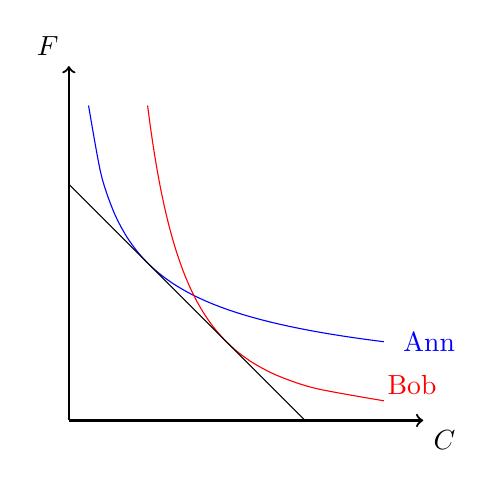
\begin{tikzpicture}[
    dot/.style={shape=circle, inner sep=2pt, draw, node contents=},
    circ/.style={shape=circle, inner sep=2pt, draw, fill}]
    \draw[thick,->] (0,0) -- (4.5,0) node[anchor=north west] {$C$};
    \draw[thick,->] (0,0) -- (0,4.5) node[anchor=south east] {$F$};
    \draw[color=blue,domain=0.25:4,smooth,variable=\x] plot ({\x},{2/sqrt(\x)}) node[label=right:{Ann}]{};
    \draw[color=red,domain=4:0.25,smooth,variable=\x] plot ({2/sqrt(\x)},{\x}) node[label=right:{Bob},yshift=2mm,xshift=-2mm]{};
    \draw (0,3) -- (3,0);  
  \end{tikzpicture}
\end{center}

\subsubsection*{c.2}

For Ann, we want that since she is better at the theory of the firm, that if $C
= F$, $MP_F > MP_C$. Then, for a general Cobb-Douglas $q(C,F) = C^\alpha
F^\beta$, we have that $ MP_F = \beta C^{\alpha}F^{\beta-1}, MP_C = \alpha
C^{\alpha-1}F^{\beta}$. When $C = F$,

\[
  MP_F > MP_C \implies \beta C^{\alpha}F^{\beta-1}> \alpha C^{\alpha-1}F^{\beta} \implies \beta > \alpha
\]

For Bob, we want that since he is better at the theory of consumer choice, that
if $C = F$, $MP_F < MP_C$.

\[
  MP_F > MP_C \implies \beta C^{\alpha}F^{\beta-1} < \alpha
  C^{\alpha-1}F^{\beta} \implies \beta < \alpha
\]

In order to reflect that they are equally good students, we want that their
total production should be equal if they have the same amount of time to spend.
Since Cobb-Douglass production functions yield the optimal technique as spending
$\frac{\alpha}{\alpha+\beta}$ of the total time spent on $C$ and
$\frac{\beta}{\alpha+\beta}$ of the total time spent on $F$, we want that for
both Ann and Bob that $\alpha_{Ann} = \beta_{Bob}, \beta_{Ann} = \alpha_{Bob}$.

Thus, we can take $q_{Ann}(C,F) = CF^2, q_{Bob}(C,F)=C^2F$.

This is also probably not a good way to actually study, in the sense that this
calculation of production is not reflective of how learning is quantified on exams.

\section*{Problem 2}

\subsection*{a)}

\begin{align*}
  q(\lambda L,\lambda K,\lambda CR) &= (\lambda L)^{0.55} (\lambda K)^{0.04} (\lambda CR)^{0.41} \\
            &= \lambda^{0.55+0.04+0.41}L^{0.55}K^{0.04}CR^{0.41} \\
            &= \lambda L^{0.55}K^{0.04}CR^{0.41} \\
            &= \lambda q(L,K,CR)
\end{align*}

We then see constant returns to scale.

However, if you only consider returns to scale relative to $L,K$, then we see
that

\[
  q(\lambda L,\lambda K) = \lambda^{0.59}q(L,K) < \lambda q(L,K)
\]

and we get decreasing returns to scale.

\subsection*{b)}

\begin{align*}
  MP_{CR} &= \frac{dq}{dCR} \\
          &= 0.41L^{0.55}K^{0.04}CR^{0.41-1} \\
          &= 0.41L^{0.55}K^{0.04}CR^{-0.59} \\
\end{align*}

\subsection*{c)}

\begin{align*}
  MRTS_{K,L} &= \frac{MP_L}{MP_K} \\
             &= \frac{0.55L^{0.55-1}K^{0.04}CR^{0.41}}{0.04L^{0.55}K^{0.04-1}CR^{0.41}} \\
             &= \frac{0.55K}{0.04L}
\end{align*}

This does not change with the level of cash reserves.

\section*{Problem 3}

\subsection*{a)}

\begin{align*}
  q(\lambda L,\lambda K) &= (\lambda L)^{0.5}\lambda K \\
                         &= \lambda^{1.5}L^{0.5}K \\
                         &> \lambda L^{0.5}K \\
                         &= \lambda q(L,K)
\end{align*}

We see increasing returns to scale, as $q(\lambda L,\lambda K) > \lambda q(L,K)$.

\subsection*{b)}

\begin{align*}
  MP_L &= \frac{dq}{dL} = 0.5L^{-0.5}K \\
  MP_K &= \frac{dq}{dK} = L^{0.5}
\end{align*}

\subsubsection*{b.1}

\[
  \min_{[L,K]} 4000L + 8000K \text{ s.t. } q = L^{0.5}K = 1000
\]
\subsubsection*{b.2,b.3,b.4}

\begin{alignat*}{2}
  && \Lag(L,K,\lambda) &= 4000L + 8000K - \lambda[L^{0.5}K - 1000] \\
  && \frac{\delta \Lag}{\delta L} &= 4000 - 0.5\lambda L^{-0.5}K = 0 \\
  && \frac{\delta \Lag}{\delta K} &= 8000 - \lambda L^{0.5} =0 \\
  && \frac{\delta \Lag}{\delta \lambda} &=L^{0.5}K  - 1000 = 0\\
  &\implies& L^{-1}K &= 1 \\
  &\implies& L &= K \\
  &\implies& K &= 1000^{0.67} = 100 \\
  &\implies& L &= 1000^{0.67} = 100
\end{alignat*}

\subsubsection*{b.5}

To see 1000 patients, we have that the minimum cost is $4000(100) + 8000(100) = 1,200,000$.

\subsection*{c)}

\begin{center}
  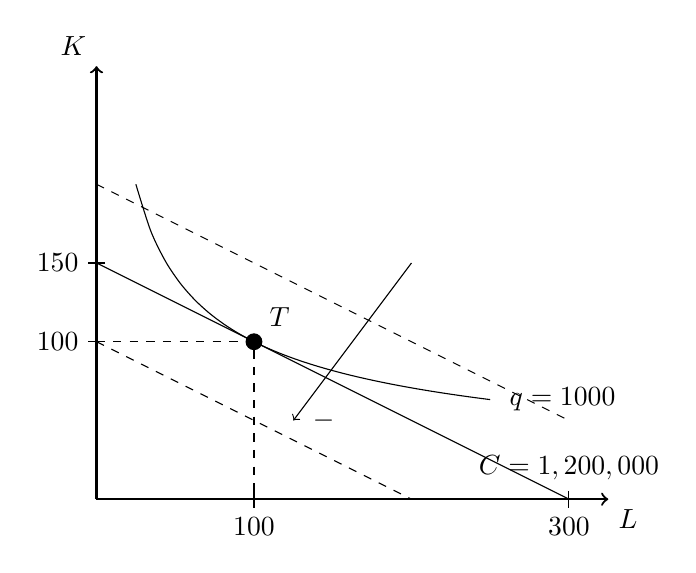
\begin{tikzpicture}[
    dot/.style={shape=circle, inner sep=2pt, draw, node contents=},
    circ/.style={shape=circle, inner sep=2pt, draw, fill}]
    \draw[thick,->] (0,0) -- (6.5,0) node[anchor=north west] {$L$};
    \draw[thick,->] (0,0) -- (0,5.5) node[anchor=south east] {$K$};
    
    \draw (6cm,3pt) -- (6cm,-3pt) node[anchor=north] {$300$}; 
    \draw (3pt,3cm) -- (-3pt,3cm) node[anchor=east] {$150$};

    \draw (2cm,3pt) -- (2cm,-3pt) node[anchor=north] {$100$}; 
    \draw (3pt,2cm) -- (-3pt,2cm) node[anchor=east] {$100$};

    \draw[domain=0.5:5,smooth,variable=\x] plot ({\x},{sqrt(8/(\x))}) node[label=right:{$q = 1000$}]{};

    \draw (2,2) node[circ,label=above right:{$T$}]{};

    \draw (0,3) -- (6,0) node[label=above:{$C = 1,200,000$}]{};
    \draw[dashed] (0,4) -- (6,1) ;
    \draw[dashed] (0,2) -- (4,0) ;
    \draw[->] (4,3) -- (2.5,1) node[label=right:{$-$}]{};
    \draw[dashed] (0,2) -- (2,2) -- (2,0);
  \end{tikzpicture}
\end{center}

\subsection*{d)}

The share on labor is equal to

\[
  \frac{\text{total spent on labor}}{\text{total costs}} = \frac{wL}{TC} =
    \frac{4000(100)}{1200000} = \frac{1}{3}
\]

Similarly, the share on capital is equal to

\[
  \frac{\text{total spent on capital}}{\text{total costs}} = \frac{wL}{TC} =
  \frac{8000(100)}{1200000} = \frac{2}{3}
\]

We notice that $q(L,K) = L^{0.5}K$, and that the share spent on labor is
$\frac{0.5}{0.5+1} = \frac{1}{3}$, and that the share spent on capital is
$\frac{1}{0.5+1} = \frac{2}{3}$.

In general, for $q(L,K) = L^{\alpha}K^{\beta}$, we have that the share spent on
labor is $\frac{\alpha}{\alpha+\beta}$ and the share spent on capital is
$\frac{\beta}{\alpha+\beta}$, matching what we know about Cobb-Douglas functions
from consumer choice.

\subsection*{e),f),g)}

These do not exist, for some reason.

\subsection*{h)}

We solve for cost minimizing $L,K$ as functions of $w,r,q$ (these are
conditional demands for $L,K$) and substitute these into the cost function.

\subsection*{i)}

\begin{align*}
  \frac{MP_L}{MP_K} &= \frac{w}{r} \\
  \frac{0.5L^{-0.5}K}{L^{0.5}} &= \frac{w}{r} \\
  \implies \frac{K}{2L} &= \frac{w}{r} \\
  \implies K &= \frac{2wL}{r} \\
  \implies q &= L^{0.5}\frac{2wL}{r} \\
                    &= L^{1.5}\frac{2wL}{r} \\
  \implies L&= (\frac{rq}{2w})^{\frac{2}{3}} \\
  \implies q &= (\frac{rq}{2w})^{\frac{1}{3}} K \\
  \implies K &= q(\frac{2w}{rq})^{\frac{1}{3}} \\
                    &= (\frac{2wq^2}{r})^{\frac{1}{3}}
\end{align*}

\subsection*{j)}

The clinic's total cost function is then $C(w,r,q) =
w(\frac{rq}{2w})^{\frac{2}{3}} + r(\frac{2wq^2}{r})^{\frac{1}{3}} =
(\frac{1}{2}rwq^{\frac{1}{2}})^{\frac{2}{3}} + (2wq^2r^2)^{\frac{1}{3}}$.

\subsection*{k)}

We have that

\begin{align*}
  AC &= \frac{C(w,r,q)}{q} \\
     &= \frac{1}{q} [(\frac{1}{2}rwq^{\frac{1}{2}})^{\frac{2}{3}} + (2wq^2r^2)^{\frac{1}{3}}] \\
     &= q^{-\frac{1}{3}}(\frac{1}{2}rw^{\frac{1}{2}})^{\frac{2}{3}} + q^{-\frac{1}{3}}(2wr^2)^{\frac{1}{3}} \\
     &= q^{-\frac{1}{3}}((\frac{1}{2}rw^{\frac{1}{2}})^{\frac{2}{3}} + (2wr^2)^{\frac{1}{3}}) \\
  \implies \frac{dAC}{dq} &= -\frac{1}{3}q^{-\frac{4}{3}}((\frac{1}{2}rw^{\frac{1}{2}})^{\frac{2}{3}} + (2wr^2)^{\frac{1}{3}}) < 0\\
\end{align*}

Thus, AC is decreasing with increased output, agreeing with our initial finding
of economies of scale.

\section*{Problem 4}

This does not exist.

\section*{Problem 5}

\subsection*{a)}

The problem here is to minimize $15L + 60K$ such that $q(L,K) =
L^{\frac{1}{3}}K^{\frac{1}{3}} = 4$.

\begin{alignat*}{2}
  && \Lag(L,K,\lambda) &= 15L + 60K - \lambda(L^{\frac{1}{3}}K^{\frac{1}{3}} -
  4) \\
  && \frac{\delta \Lag}{\delta L} &= 15 - \frac{1}{3}\lambda
  L^{\frac{-2}{3}}K^{\frac{1}{3}} = 0\\
  && \frac{\delta \Lag}{\delta L} &= 60 - \frac{1}{3}\lambda
  L^{\frac{1}{3}}K^{\frac{-2}{3}} = 0\\
  && \frac{\delta \Lag}{\delta \lambda} &= L^{\frac{1}{3}}K^{\frac{1}{3}} - 4
  =0 \\
  &\implies& \frac{60}{15} &= \frac{L}{K}  \\
  &\implies& 4K &= L \\
  &\implies& 4^{\frac{1}{3}}K^{\frac{2}{3}} &= 4 \\
  &\implies& K &= 4, L = 16
\end{alignat*}

\subsection*{b)}

The firm's total cost is then $15(16) + 60(4) = 240 + 240 = \$480$.

\subsection*{c),d)}

\begin{center}
  \begin{tikzpicture}[
    dot/.style={shape=circle, inner sep=2pt, draw, node contents=},
    circ/.style={shape=circle, inner sep=2pt, draw, fill}]
    \draw[thick,->] (0,0) -- (8.5,0) node[anchor=north west] {$L$};
    \draw[thick,->] (0,0) -- (0,8.5) node[anchor=south east] {$K$};

    \draw (8cm,3pt) -- (8cm,-3pt) node[anchor=north] {$32$}; 
    \draw (3pt,2cm) -- (-3pt,2cm) node[anchor=east] {$8$};
    \draw (4,1) node[circ,label=above right:{$T$}]{};

    \draw[domain=2:32,scale=0.25,smooth,variable=\x] plot ({\x},{64/\x}) node[label=right:{$q = 4$}]{};
    \draw (0,2) -- (8,0) node[label=above right:{$TC=480$},xshift=-20mm,yshift=-2mm]{};

    \draw (4cm,3pt) -- (4cm,-3pt) node[anchor=north] {$16$}; 
    \draw (3pt,4cm) -- (-3pt,4cm) node[anchor=east] {$16$};
    \draw (2,2) node[circ,label=above right:{$T'$}]{};

    \draw (0,4) -- (4,0) node[label=above right:{$TC' = 240$},xshift=-10mm]{};

    \draw (2cm,3pt) -- (2cm,-3pt) node[anchor=north] {$8$}; 
    \draw (3pt,1cm) -- (-3pt,1cm) node[anchor=east] {$4$};

    \draw[dashed] (0,2) -- (2,2) -- (2,0);
    \draw[dashed] (0,1) -- (4,1) -- (4,0);

    % \draw (3pt,8cm) -- (-3pt,8cm) node[anchor=east] {$32$};
    % \draw (2,2) node[circ,label=above right:{$T'$}]{};

    % \draw (0,8) -- (8,0) node[label=right:{$TC' = 480$},xshift=-5mm,yshift=10mm]{};
    % \draw[domain=4:16,scale=0.5,smooth,variable=\x] plot ({\x},{64/\x}) node[label=right:{$q = 4$}]{};
  \end{tikzpicture}
\end{center}

Note that after the subsidy, we have that $\frac{MU_K}{MU_L} = \frac{15}{15}
\implies \frac{L}{K} = 1 \implies L = K = 8$.

\subsection*{e)}

The total cost is diminished to $15L + 15K = 15(8) + 15(8) = \$240$.

\subsection*{f)}

This situation is different from consumer choice in the sense that the firm's
output does not actually change with the subsidy, meaning that the government is
just paying for no extra production. The welfare benefit to the producer then is
simply the reduction in costs of $\$240$.

This subsidy's cost is given by the fact that the firm utilizes 16 units of $K$, each
subsidized at $\$45$ each, for a total cost of $16(45) = 720$. The final excess
burden then is $720 - 240 = 480$.

Morally, this is also the same as excess burden in consumer choice as that
considered the situation where a lump sum incurring the same welfare loss would
raise more tax revenue; in this case, a flat subsidy of $\$240$ would have
sufficed, but the per unit subsidy on $K$ incurs an extra $\$480$ of government spending.

\subsection*{g)}

% If we have a long run evolution of factor productivity like this, then we would
% see that the subsidy increases total factor productivity by a factor of two
% every year compared to the world where the subsidy is not enacted (This can be
% seen from the fact that the conditions of $L = 4K$ without the subsidy and $L =
% K$ with the subsidy are kept irregardless of overall factor productivity). Thus,
% if the subsidy is in place for $n$ years, then overall factor productivity will
% be higher by a factor of $2^n$ than if the subsidy never existed.

If we have a long run evolution of factor productivity like this, then we would
see that the subsidy increases total factor productivity to a higher degree than
without the subsidy. For example, after the first year ($q_0 =
L^{\frac{1}{3}}K^{\frac{1}{3}}$), we would see that $q_1 =
8L^{\frac{1}{3}}k^{\frac{1}{3}}$ in the presence of the subsidy and $q_1 =
4L^{\frac{1}{3}}K^{\frac{1}{3}}$ without.

The case with the subsidy, the firm would spend for $L = K =
\frac{1}{2\sqrt{2}}$ units for a total cost of $\frac{1}{\sqrt{2}} \cdot 15 =
\frac{15}{\sqrt{2}}$, whereas without the subsidy the firm would spend for $L =
K = 1$ for a total cost of $15\cdot 2 = 30$.

Then, the subsidy has now totaled spending of $720 + 45(\frac{1}{2\sqrt{2}}) =
736$, a small increase after the first year. Comparatively, the firm has only
spent $240 + \frac{15}{\sqrt{2}} = 251$, as compared to $480 + 30 = 510$ without
the subsidy. The excess burden is then $736 - (510-251) = 477$, which has
diminished from before, indicating that the subsidy is actually positive for the
second year, drastically increasing the efficacy of the policy.

After the first few years, $q_t$ is harder to predict as it is not $q_t =
\frac{K_{t-1}}{2}q_{t-1}$, which would make it easier to solve, but still
generally have the subsidy as more effective than in the first year (i.e.
incurring less excess burden).

\end{document}